\section{Related work} \label{related_work}
This chapter goes over all prior knowledge that is required to properly follow the rest of this thesis. We quickly go through some fundamentals of rendering, and quickly move to volume rendering specific topics. We conclude this Chapter with the gaps in current research and where this research fits in.



\begin{wrapfigure}{r}{0.4\textwidth}
    \centering
    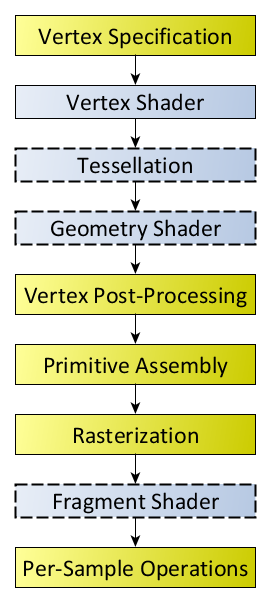
\includegraphics[width=0.5\linewidth]{figures/rasterization_pipeline.png}
    \caption{An overview of the rasterization pipeline, where blue stages are programmable and yellow stages are dedicated stages built into GPU hardware. We start with a bunch of vertices and apply a vertex shader. This allows the triangles to be transformed for whatever reason, whether it's because the camera was moved or an object has changed for example. Then we tessellate the vertices into triangles. After which we apply an optional geometry shader that can generate or remove triangles. Then our triangles are projected onto an image, and we end up with information like normal, texture coordinate, and depth. This information can then be used to calculate the final color of a certain set of pixels. \cite{RasterPipeline}}
    \label{fig:rasterization_pipeline}
\end{wrapfigure}


\subsection{Rendering in games} \label{related_work:rendering}
Computers have existed for some time now, and since the start, they have been used to render things on a screen. Whether this is text, graphs, photos, or virtual worlds. When rendering virtual worlds, for example, games or movies, optimized algorithms have to be used to keep up with the growing complexity and increasing fidelity that is expected of new titles. One of these algorithms that has been used in practically all games is rasterization, which quickly projects triangles onto the screen. A different algorithm, with different benefits and drawbacks, is ray tracing, which tries to emulate the physical properties of light as it exists in the real world. Usually, we render scenes that consist of a set of models, for example for every tree, rock or character in the world. These models are made up of triangles which store details such as material, normal and position.


\subsubsection{Rasterization} \label{related_work:rendering:rasterization}
Screen space rendering techniques using the graphics processing unit's (GPU) hardware rasterizer are frequently referred to as rasterization. This technique has been the industry standard for at least the past 20 years. It is a pipeline of operations that calculates which triangles are visible (see Figure \ref{fig:rasterization_pipeline}). Because graphics hardware has been optimized for this specific pipeline, it is fast and thus, if possible, the rasterization pipeline can and should be exploited where possible. However, there are issues. For example, reflections can not show off-screen objects without sophisticated (and often slow) tricks. This is an inherent issue with the rasterization because the fragment shader stage does not know anything about off-screen and obscured triangles. Along with that, rasterization performance scales linearly with the number of triangles. Therefore, it quickly becomes impractical to use for scenes/assets with incredibly high triangle counts, as required by modern render pipelines.

\subsubsection{Ray and path tracing} \label{related_work:rendering:ray_tracing}
Ray tracing is an entirely different technique that allows us to create arbitrary rays and find what primitives they intersect. Which has the benefit of no longer being bound to a certain view matrix, like with rasterization. This immediately opens up the door for techniques that were traditionally not possible. For example, off-screen reflections can now be rendered by shooting new rays from the reflection point (see Figure \ref{fig:path_ray_raster}). We also don't have to process every triangle individually, instead, we can shoot rays for every pixel in the screen, and find the intersecting triangles quickly.

Although ray tracing has been theorized by many to be the replacement of classic rasterization methods, we have only recently seen it being applied to games after NVIDIA released its RTX graphics cards. Additionally, we see that all AAA games currently still depend on the rasterizer and only use ray tracing to enhance their graphics either by adding realistic (1) diffuse indirect light, which is often mislabeled as global illumination, (2) shadows, (3) reflections, (4) ambient occlusion or a combination of these four\cite{NVIDIARTX}.
\begin{figure}[H]
    \centering
    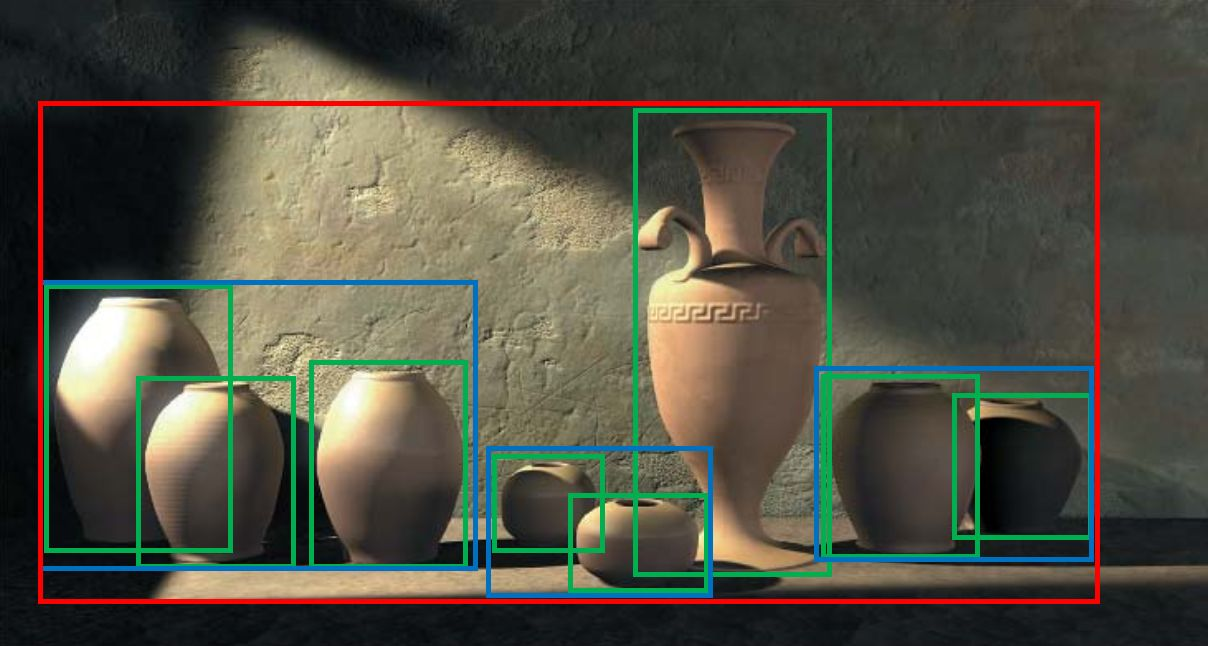
\includegraphics[width=0.9\linewidth]{figures/bvh.jpg}
    \caption{A bounding volume hierarchy where the red bounding box encapsulates all objects. Then a step lower in the hierarchy, we see the blue bounding boxes which encapsulate groups of objects. And the leaves, indicated by the green bounding boxes, contain the primitives. These structures are stored in a tree-like structure and can, theoretically, have infinite depth or width. Finding the intersection between a ray and the bounding volume hierarchy can be done in $O(\log n)$ time on average, where n is the number of primitives. \cite{BVHJacco}}
    \label{fig:bvh}
\end{figure}

Path tracing is a specific algorithm that uses ray tracing to calculate physically accurate images by trying to solve the rendering equation \cite{kajiya1986rendering}. It does this by using recursive numerical integration of the rendering equation for every pixel. This results in a realistic image once converged. However, for the longest time, this has been too slow to run in real-time on commodity hardware. Fortunately, there have been some major advances in (1) sampling techniques as described in \cite{lin2022generalized} and (2) filtering techniques as described in \cite{yang2020survey}. Along with the advent of better GPU hardware, it might make real-time path tracing a reality for upcoming AAA games.

\begin{wrapfigure}{r}{0.4\textwidth}
    \centering
    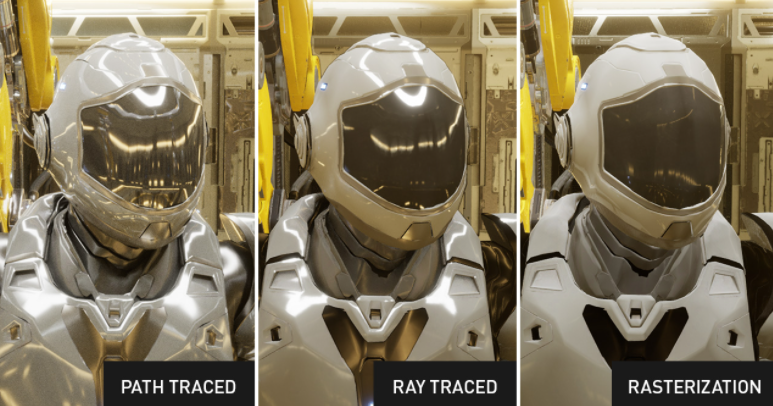
\includegraphics[width=\linewidth]{figures/nvidia_ray_path_rasterization.png}
    \caption{Here we see the difference between a path traced, a ray-traced and a rasterized render. As can be seen, the rasterized scene does not contain accurate reflections and has trouble with specular highlights from the many lights. The ray-traced render does show accurate specular reflections. And when we look at the path traced scene we also see glossy reflections and accurate indirect illumination. \cite{NVIDIAPathRayRaster}}
    \label{fig:path_ray_raster}
\end{wrapfigure}

Generally, path tracing involves multiple steps to achieve real-time performance \cite{laine2013megakernels}, (1) ray generation, (2) ray extension, (3) shading and (4) shadow ray extension. This pipeline is executed for every pixel on the screen, so for a standard 1080p monitor that would be $1920*1080=2.073.600$ rays. Step 1 is executed once at the start, and then the latter three steps are done repeatedly to simulate realistic light transport through the scene. The main task of steps 2 and 4 is to find intersections with the scene geometry. This can be done by individually performing intersection tests with every triangle in the scene with a time complexity of $O(n)$, where $n$ is the number of triangles. However, this linear scaling is prohibitive when the complexity of models increases. So to fix this problem, bounding volume hierarchies (BVH as seen in Figure \ref{fig:bvh}) are used to accelerate these intersection tests. This is done by creating a traversable tree with triangles at the leaf nodes, which reduces the average traversal time to  $O(\log n)$. To allow instanced rendering without drastically increasing the triangle count of the scene or increasing build times, a top-level acceleration structure (TLAS) is created over a bottom-level acceleration structure (BLAS). Here the TLAS contains pointers to multiple BLAS's which contain the actual model data \cite{VulkanAccelerationStructures}.

\subsection{Path traced volume rendering} \label{related_work:path_traced_volume_rendering}
In this project volume data represents clouds, explosions, fire and sand/dust storms. This means that we are not just interested in finding the discretized boundary of a volume, but also in the contents of the volume. We may have varying densities or even different materials within one volume. For example, a flame that emits light surrounded by smoke, where the outer edge of this smoke is so sparse that it is almost completely transparent. When shading these kinds of materials there are three main things which can happen: (1) The ray is absorbed, meaning that no light transport will be rendered. When this happens, the light energy is converted into another energy form like heat. (2) The ray is traversed through (refracted) or bounces off (reflected) the particle. This will change the direction of the ray and potentially change the ray payload, for example when a blue particle is hit, the ray is modified to only return the blue color if a light is hit. (3) The ray hits an emissive particle. Meaning that light transport will be rendered, and the ray will not continue.

\subsubsection{Data structure} \label{related_work:path_traced_volume_rendering:data_structure}
Ray tracing these kinds of volumes is different from normal ray tracing, as they require completely different methods. Normally there is a set of surfaces that define a scene. To render these scenes, BVHs are used to find an intersection between a ray and the scene as described in Section \ref{related_work:rendering:ray_tracing}. For volume rendering, we don't have these concrete surfaces but instead have volumes with implicit particles, like dust or water droplets from a cloud. To render these volumes we somehow have to find where we hit such a particle and evaluate its shading function. We do not simulate these particles individually but describe volumes of the scene using densities, which are discretized into small volumetric pixels (voxels).

\subsubsection{Delta tracking} \label{related_work:path_traced_volume_rendering:delta_tracking}
When traversing such a volume we calculate how far we can traverse through these densities before we are likely to hit a particle. Then we take the step, evaluate the shading function and calculate how long our next step can be. This process is called ray marching \cite{RenderingWithTwoTriangles}. For homogeneous volumes (with a uniform density) these step sizes will always be the same, but for heterogeneous volumes, they might not. In the heterogeneous case, we calculate the longest possible step we could take through the most dense voxel in our scene and use that to make sure we do not overshoot and miss any dense voxels. This method is called delta tracking \cite{kutz2017spectral} and quickly becomes expansive when a single voxel has a high density. A solution would be to take steps proportional to the highest local density, for example, the highest density of the $8^3$ nearest voxels. This way we can take step sizes that are proportional to the densities which we are currently traversing, instead of crippling the performance for every ray because of a single voxel.

\begin{figure}[H]
    \centering
    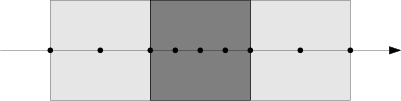
\includegraphics[width=0.9\linewidth]{figures/sample_step_size.png}
    \caption{A ray traversing through a heterogeneous volume, where dots represent the location of shading evaluations. As can be seen, the more dense the volume (darker) the shorter the steps are.}
    \label{fig:sample_step_size}
\end{figure}

\begin{wrapfigure}{r}{0.4\textwidth}
    \centering
    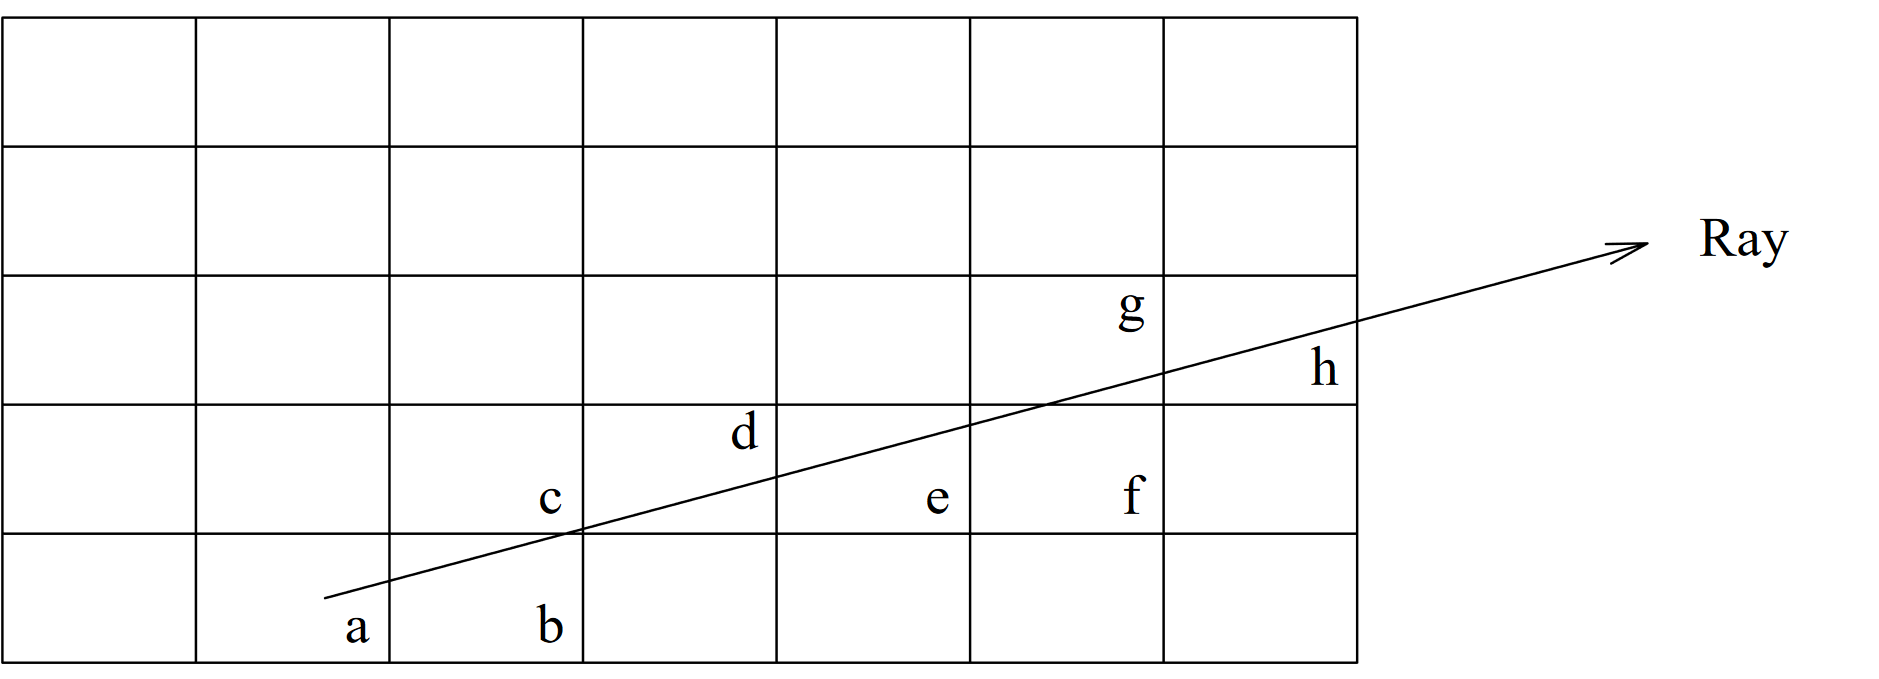
\includegraphics[width=\linewidth]{figures/dda.png}
    \caption{A ray being shot through a dense grid and marking every traversed voxel with a letter. \cite{amanatides1987fast}}
    \label{fig:dda_traversal}
\end{wrapfigure}

\subsection{Voxel data structures} \label{related_work:voxel_data_structures}
Data structures for volume data have seen multiple forms trying to optimize ray marching performance, memory footprint, update speed and simplicity. This research specifically targets heterogeneous volumes which often consist of gradients where outer voxels can have small non-zero values, instead of having opaque volume boundaries. We will briefly go over some major volume data structures, below.

\begin{wrapfigure}{r}{0.4\textwidth}
    \centering
    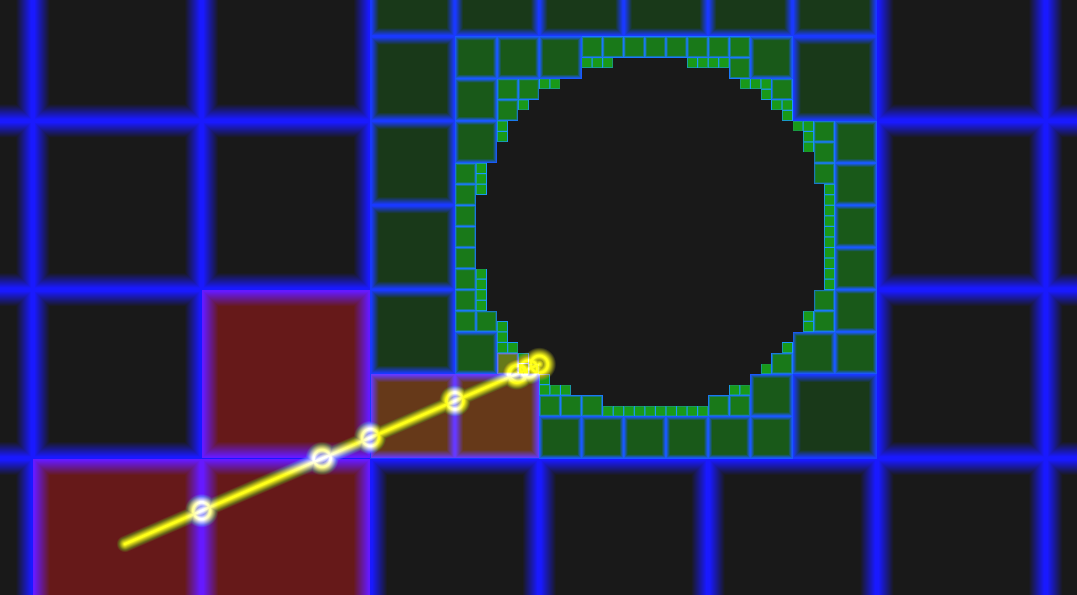
\includegraphics[width=\linewidth]{figures/esvo_traversal.png}
    \caption{Hierarchical digital differential analyzer (HDDA) traversal through a sparse voxel octree. The yellow line is our ray. The brighter green a cell is, the deeper our nodes in the octree are. We can see that nodes that are further away from the circle, can be stepped through with big steps, but as we approach the circle, our steps become smaller. \cite{ShaderToyQuadtree}}
    \label{fig:esvo}
\end{wrapfigure}




\subsubsection{Dense 3D grid} \label{related_work:voxel_data_structures:dense_grid}
The most basic structure (see Figure \ref{fig:dda_traversal}). Here, every value in the 3D array corresponds to a voxel. Indexing into this structure is fast and editing is trivial. However, there is no compression or space skipping. Another problem with flat arrays is their memory requirement as it has cubic scaling with the resolution. However, small-scale simulation software still often relies on this data structure as it is easy to implement, and in many cases, simulations have to update each voxel anyway.



\subsubsection{Efficient sparse voxel octrees (ESVO)} \label{related_work:voxel_data_structures:esvo}
A solution to the memory problems was proposed by NVIDIA, by introducing sparsity to homogeneous volume data \cite{laine2010efficient}. The main contribution is a data structure that drastically reduces the memory footprint by not storing information about homogeneous areas. This memory reduction also yields a speedup when traversing the volume, as larger steps can be taken through homogeneous areas (see Figure \ref{fig:esvo}). Along with that, the structure will more easily fit in the different caches of the GPU. However, due to the nature of tree structures, the data access pattern is less coherent which negatively impacts ray marching performance. The paper also did not take any form of animation into account. So this data structure only really works on static scenes \cite{JohnLinPerfectEngine}.


\subsubsection{Sparse voxel directed acyclic graphs} \label{related_work:voxel_data_structures:svdag}
A follow-up paper was released further improving the memory footprint optimization \cite{kampe2013high}. Here, the nodes of the octree can be reused for identical volumes, so one leaf can be the child of multiple nodes that share the same data (see Figure \ref{fig:DAG_node_deduplication}). The result is a significant reduction in memory usage over ESVO. Afterward, additional papers were written to, (1) further optimize the memory footprint by creating a lossy data structure which will slightly alter the volume data in an attempt to find more similar volumes \cite{van2020lossy} (LSVDAG). And (2) allow for real-time editing of this data structure \cite{careil2020interactively} (HashDAG).

\begin{figure}[H]
    \centering
    \subfloat[Removal of identical nodes in all levels of a binary tree. In the SVDAG paper, the same technique is applied to octrees. \cite{kampe2013high}]{
        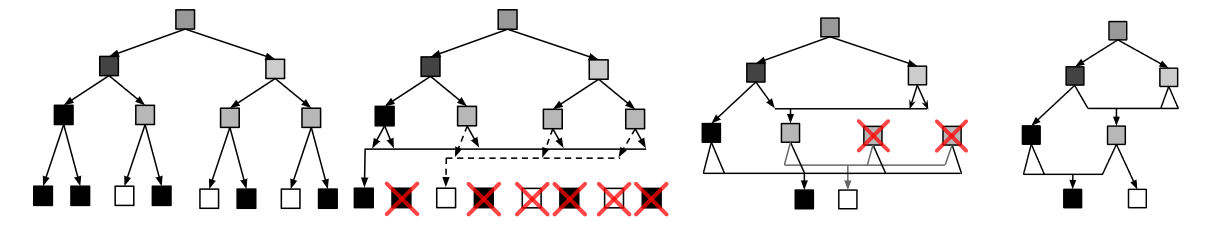
\includegraphics[width=0.45\textwidth]{figures/DAG_node_deduplication.png} \label{fig:DAG_node_deduplication}
    }
    \hfill
    \subfloat[Here we see the brick map (in red), which is dense. Whenever an area in this brick map is not homogeneous (indicated by the filled-in squares), we point to a brick (in blue). \cite{van2015real}]{
        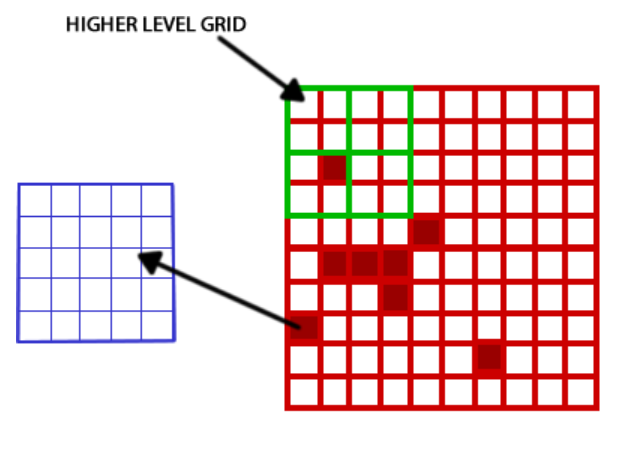
\includegraphics[width=0.45\textwidth]{figures/brickmap.png} \label{fig:brickmap}
    }
\end{figure}

\subsubsection{Brick map} \label{related_work:voxel_data_structures:brickmap}
Later another paper was released which tried to maintain part of the memory benefits from octrees while also improving ray marching performance \cite{van2015real}. This was done by keeping the idea of a hierarchical structure, but limiting the tree depth to 2 layers (a top-level grid, the brick map and the bottom-level bricks, as can be seen in Figure \ref{fig:brickmap}), which improves cache utilization. An additional benefit of reducing the depth of a data structure is the update time. When running a fluid simulation, which has to touch every leaf node in a tree, a shallower tree will take fewer steps when going down to the bottom of the tree to modify each voxel. Similar to the flat 3D array, the brick map structure is fast when it comes to update speeds, as both have shallow tree structures. Another paper explores implicit brick maps \cite{niessner2013real}. These are implicit because they don't encode their location in a grid, but hash a world position and use that hash to index into the brick buffer directly. This allows for an unbounded index space instead of having to create a grid inside a certain axis-aligned bounding box (AABB). However, nothing has been documented about them in the context of ray tracing.


\subsubsection{VDB} \label{related_work:voxel_data_structures:vdb}
In the movie industry, \textbf{VDB} \cite{museth2013vdb} has been the standard for volumetric rendering for a long time. This is a hierarchical B+tree structure with 3 layers (see Figure \ref{fig:VDB}), which optimizes for both query speed and memory size. It does so by making clever use of bit masks (see Section \ref{related_work:attribute_separation:bitmasks}), logical bitwise operations and inverted tree traversal. The last of these optimizations means that we don't have to traverse down the tree every time we query a point. But instead, we assume that consecutive points will be close to each other, and remember where we are in the tree. Then the next time we query a point we start at the bottom of the tree and have $O(1)$ access time if we retrieve a point that resides in the same bottom layer.

The VDB structure has mostly been used on the CPU. There have been implementations that port VDB to the GPU, but these do not support dynamic topology \cite{hoetzlein2016gvdb} \cite{museth2021nanovdb}. They would allow individual voxels to be modified, but can't place new voxels in arbitrary locations. This limitation makes simulation on the GPU impractical while maintaining the sparsity which makes the structure effective. The reason why this dynamic topology has never been implemented likely has to do with an inherent race condition when trying to modify any tree structure in parallel.

Research has also been conducted on encoding voxels or even internal layers of the VDB structure in neural networks \cite{kim2022neuralvdb}. These neural encodings can store a lot of detail in limited memory, but take minutes to train. Which, again, makes dynamic updates impossible.

One useful result of the standardization of VDB technology is the data format. Many tools can interface directly with the VDB file format \cite{VDBADeepDive}, and many artistic tools can export to the VDB file format. These features make it easy to download specific effects and test in a specific renderer.

\begin{wrapfigure}{r}{0.4\textwidth}
    \centering
    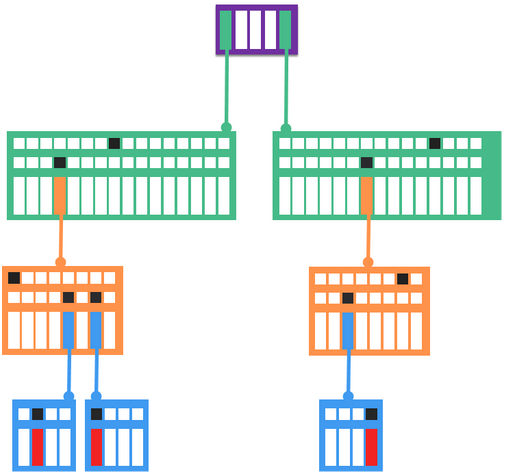
\includegraphics[width=\linewidth]{figures/OpenVDB.png}
    \caption{The four-level tree structure of the VDB data structure. In purple, we see the top node which has an arbitrary size and points to the first level of internal nodes. The two levels of internal nodes (in green and orange) both contain three rows of values. The top row is a bit mask indicating which values are "active" (this is application-specific), the middle row is a bit mask indicating that a child node exists, and the bottom row contains a pointer to the child node. Then in blue, we have a top row which is a bit mask indicating if a voxel is empty, and the bottom row containing the actual voxel data. \cite{museth2013vdb}}
    \vspace{-30pt}
    \label{fig:VDB}
\end{wrapfigure}




\subsection{Attribute separation} \label{related_work:attribute_separation}
All modern processors are built with cache hierarchies. These caches are usually a few megabytes and consist of many 128-byte cache lines. Which contain all recent memory accesses so, they can be reused quickly when the memory is fetched again. When accessing any memory, an entire cache line (of 128 bytes) is loaded. This means the memory access cost of fetching a single floating point value ($4$ bytes) is the same as fetching 32 ($128/4$) floating point values. Abusing this is key to writing fast CPU and GPU code. Therefore, it is crucial to have as little unused data within each cache line fetch as possible. This can be achieved by separating the voxel data from the geometry structure \cite{dado2016geometry}.
\subsubsection{Fast volume traversal} \label{related_work:attribute_separation:fast_volume_traversal}
There are two main branches of volume traversal. The first is by sampling the volume along a ray with certain step sizes. This is what delta tracking does (see Section \ref{related_work:path_traced_volume_rendering:delta_tracking}). Another method of traversing the volume is a more exact technique called digital differential analyzer (DDA) \cite{amanatides1987fast}. This analytically calculates how far along the ray we can step to arrive at the next voxel. Using this technique we also know exactly how much density we accumulated along our steps. This has benefits for the shading part of our render, but we won't go into that in this research. DDA has been extended to allow hierarchical volume data structures to be traversed, this is called a hierarchical digital differential analyzer (HDDA)\cite{laine2010efficient}.


Recently, NVIDIA has done research about using signed distance fields (SDF) to speed up traversal\cite{soderlund2022ray}. The general idea behind these distance fields is that the maximum step length a ray could take in any direction (without hitting anything) is pre-calculated, and used to skip over voxels that are known to be empty (see Figure \ref{fig:SDF_marching}). This method could be applied to most of the data structures described above, and might specifically be promising when combined with flat structures which don't implicitly store distance values by using bigger nodes in homogeneous volumes. However, calculating these SDFs is one additional step in the pipeline. Although this can be done quickly even for large volumes (less than $1$ ms for $1024^3$ voxels \cite{cao2010parallel}), it is unclear if the speedup during tracing outweighs the construction cost.
\subsubsection{Bit  masks} \label{related_work:attribute_separation:bitmasks}
When taking steps along a ray, there is a high chance that we will often access voxels that are close to each other, especially when using DDA, and we have to traverse all consecutive voxels. To reduce the bandwidth requirement of these methods we can use bit masks to indicate whether voxels are empty \cite{van2015real}\cite{museth2013vdb}. When using 32-bit floating point values as densities, for example, we can traverse all voxels that have a density of $0$ using the bit mask. Respectively, we can have a $16\times8\times8$ region of voxels in a single cache line, making our traversal significantly less bandwidth-heavy.

\begin{wrapfigure}{r}{0.4\textwidth}
    \centering
    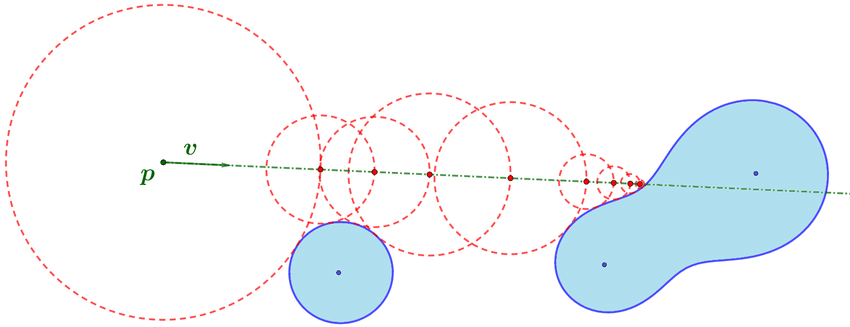
\includegraphics[width=0.9\linewidth]{figures/sdf_ray_marching.png}
    \caption{Marching through a signed distance field enables steps that are exactly as long, as the closest heterogeneity is far away. Here we see the ray in green, and the step sizes are indicated by the red circles. \cite{SDF_sphere_marching}}
    \label{fig:SDF_marching}
\end{wrapfigure}

\begin{table}[htbp]
    \centering
    \begin{adjustbox}{max width=\textwidth}
        \begin{tabularx}{\textwidth}{|c|X|X|X|X|X|}
            \hline
            \textbf{Method} & \textbf{Sampling Performance} & \textbf{DDA Performance} & \textbf{Memory Footprint} & \textbf{Update Speed} & \textbf{Simplicity} \\
            \hline
            Dense Grid      & \Plus \Plus                   & \Minus \Minus            & \Minus \Minus             & \Plus \Plus           & \Plus \Plus         \\
            \hline
            ESVO            & \Minus \Minus                 & \Plus                    & \Plus                     & \Minus \Minus         & \Minus              \\
            \hline
            SVDAG           & \Minus \Minus                 & \Plus                    & \Plus \Plus               & \Minus \Minus         & \Minus \Minus       \\
            \hline
            Brick map       & \Plus                         & \Plus \Plus              & \Minus                    & \Plus                 & \Plus               \\
            \hline
            VDB             & \Plus                         & \Plus \Plus              & \Plus                     & \Minus                & \Minus              \\
            \hline
        \end{tabularx}
    \end{adjustbox}
    \caption{An overview of the different data structures. The pluses and minuses provide some intuition into what every structure is optimized for. A very broad summary of the different metrics: The shallower the tree, the faster our sampling. Deeper trees have better DDA performance (see Section \ref{related_work:attribute_separation:fast_volume_traversal} for a very brief description), but we get optimal performance when our nodes approximate the size of our caches and cache lines. Deeper trees improve memory footprint and deduplication improves it even further. The shallower our tree, the faster and easier our updates. And simplicity depends on the method.}
    \label{tab:structure-comparison}
\end{table}

\subsection{Texture compression} \label{related_work:texture_compression}
Although it might sound odd, we could learn a thing or two from texture compression techniques. They are similar to our voxel data in the sense that both contain floating point arrays. The only two differences are that textures usually store color data and are two-dimensional, while our volume data contains densities and is three-dimensional. These floating point arrays that textures use have pretty much always been too big for computers, at least when no compression is applied. Usually, photos are compressed using a lossy technique like JPEG, and logos or other digital assets without too many gradients are compressed using PNG which is not lossy. These methods work fine when we care about compression ratios, but they do not when we want to do billions of texture fetches per second on the GPU. For this purpose block compression is usually being used\cite{BlockCompression}. Block compression has different formats for different use cases. For example, BC4 is suitable for grayscale textures, and BC5 is optimal for normals (as seen in Table \ref{tab:block_compression}). These formats all encode $4\times 4$ pixels into a certain number of bytes, which can be used for 2D textures but also technically work in three dimensions. However, we do get spatial dependencies in two out of three axes then, these are the dimensions in which the $4\times 4$ chunk is arranged.

\begin{table}[htbp]
    \centering
    \adjustbox{max width=\textwidth}{
        \begin{tabular}{|c|c|c|p{5cm}|}
            \hline
            \textbf{Type} & \textbf{Data Rate}         & \textbf{Palette Size} & \textbf{Use For}                     \\
            \hline
            BC1           & RGB + optional 1-bit alpha & 0.5 byte/px           & Color maps                           \\
                          &                            &                       & Cutout color maps (1-bit alpha)      \\
                          &                            &                       & Normal maps, if memory is tight      \\
            \hline
            BC2           & RGB + 4-bit alpha          & 1 byte/px             & n/a                                  \\
            \hline
            BC3           & RGBA                       & 1 byte/px             & Color maps with full alpha           \\
                          &                            &                       & Packing color and mono maps together \\
            \hline
            BC4           & Grayscale                  & 0.5 byte/px           & Height maps                          \\
                          &                            &                       & Gloss maps                           \\
                          &                            &                       & Font atlases                         \\
                          &                            &                       & Any grayscale image                  \\
            \hline
            BC5           & 2 $\times$ grayscale       & 1 byte/px             & Tangent-space normal maps            \\
            \hline
            BC6           & RGB, floating-point        & 1 byte/px             & HDR images                           \\
                          &                            &                       &                                      \\
            \hline
            BC7           & RGB or RGBA                & 1 byte/px             & High-quality color maps              \\
                          &                            &                       & Color maps with full alpha           \\
            \hline
        \end{tabular}
    }
    \caption{Block compression formats and use cases \cite{BlockCompression}.}
    \label{tab:block_compression}
\end{table}




\subsection{Gaps in current research} \label{related_work:gaps_in_current_research}
There are of course still many issues with volume data structures, so below are some of the most notable issues with the current state-of-the-art, and how we can push the state-of-the-art forward in a meaningful way. Many methods have either optimized volume data structures for memory usage \cite{laine2010efficient}\cite{kampe2013high}, ray tracing performance \cite{van2015real} \cite{soderlund2022ray} \cite{museth2013vdb} or simulation times (flat 3D array). However, none of these techniques currently can do all three of these things while keeping all data and computation on the GPU. Below are two issues that this research tries to address.
\subsubsection{Large assets} \label{related_work:gaps_in_current_research:large_assets}
Video game assets have been growing in size to the point where games can be hundreds of gigabytes. Adding another asset type, volumes would further increase this. So although there has been a lot of research done in compressing geometry (the volume shape without its per voxel attributes) to the point where entire scenes can be voxelized into game-ready asset sizes\cite{van2015real}\cite{museth2013vdb}. We also need our actual density data to be small, which has been done by \cite{dado2016geometry}, but this was applied to normals and colors, not specifically densities which only have one floating point value per voxel instead of three.
\subsubsection{Animation delta compression} \label{related_work:gaps_in_current_research:animation_delta_compression}
Another thing that has not been explored extensively is applying delta compression on our volumes. This has been hinted at by \cite{careil2020interactively}, where they suggest encoding animation frames as different branches of the tree. Resulting in a structure that can simply swap some pointers at certain points in the tree when changing to the next frame. However, there are two issues with this method: (1) The deep quad-tree structure is not optimized for tracing, and when flattening the structure we rapidly reduce the effectiveness of deduplicating our nodes. (2) This does not change the attributes of the lower-level nodes, so when our attributes change (a density increases or decreases) we would have to swap pointers high up in the tree, effectively requiring a new tree for every animation frame.